\section{Criar Módulo} %%%%%%%%%%%%%%%%%%%%%%%%%%%%%%%%%%%%%%%%%%%%%%%%%%%%%%%

\subsection*{Instalação} %%%-----------------------------------------

\begin{frame}[fragile]
	\frametitle{Preparação do ambiente}
	
	\begin{itemize}
		\item<1-> Primeiro temos que instalar e preparar os \textit{headers} do \textit{kernel}:
	\end{itemize}

	\lstset{language=bash}

	\begin{block}<1->{}
	\begin{lstlisting}
		sudo -i
		apt-get install module-assistant
		m-a prepare
	\end{lstlisting}
	\end{block}

	\begin{itemize}
		\item<2-> Obs.: O seguinte comando também instala os pacotes que precisamos (equivalente ao ``m-a prepare''):
	\end{itemize}

	\begin{block}<2->{}
	\begin{lstlisting}
		sudo apt-get install build-essential linux-headers-$(uname -r)
	\end{lstlisting}
	\end{block}

\end{frame}


\begin{frame}[fragile, allowframebreaks]
	\frametitle{Arquivo fonte \nocite{}}
	\begin{itemize}
		\item<1-> Crie um diretório e insira o arquivo `hello.c' \cite{KernelDevelopment} \cite{HelloWorld_Mark}, contendo o seguinte código:
	\end{itemize}
	\lstset{frame=lines}
	\lstinputlisting[language=C]{hello.c}
\end{frame}


\begin{frame}[fragile]
	\frametitle{Makefile \nocite{}}
	\begin{itemize}
		\item<1-> Crie o arquivo `Makefile' \cite{HelloWorld_Mark} com as seguintes informações:
	\end{itemize}
	\lstset{frame=lines}
	\lstinputlisting[language={[gnu]Make}]{Makefile.}
\end{frame}


\begin{frame}[fragile]
	\frametitle{Compilar o código}
	
	\begin{itemize}
		\item<1-> Para compilar o código basta executar o `make':
	\end{itemize}

	\begin{block}<1->{}
	\lstset{language=bash}
	\begin{lstlisting}
		make
	\end{lstlisting}
	\end{block}

	\pause

	\begin{itemize}
		\item<1-> Exemplo de retorno do comando `make':
	\end{itemize}

	\lstset{language=TeX, numbers=none}
	\begin{lstlisting}
		make -C /lib/modules/3.2.0-4-686-pae/build M=/home/anderson/modulos modules
		make[1]: Entrando no diretorio `/usr/src/linux-headers-3.2.0-4-686-pae'
		  Building modules, stage 2.
		  MODPOST 1 modules
		make[1]: Saindo do diretorio `/usr/src/linux-headers-3.2.0-4-686-pae'
	\end{lstlisting}

\end{frame}


\begin{frame}[fragile]
	\frametitle{Inserir/Remover Módulo}
	
	\begin{itemize}
		\item<1-> Para inserir o novo módulo no \textit{kernel}:
	\end{itemize}

	\lstset{language=bash}

	\begin{block}<1->{}
	\begin{lstlisting}
		sudo insmod hello.ko
	\end{lstlisting}
	\end{block}

	\begin{itemize}
		\item<2-> Para remover o módulo do \textit{kernel}:
	\end{itemize}

	\begin{block}<2->{}
	\begin{lstlisting}
		sudo rmmod hello
	\end{lstlisting}
	\end{block}

\end{frame}


\begin{frame}
	\frametitle{Inserir/Remover Módulo}
	\begin{itemize}
		\item<1-> Ligando um módulo ao \textit{kernel}:
		\note[item]<1> {gendisk - Representação do disco no Kernel}
		\note[item]<1> {block_device_operations - Conjunto de operações do dispositivo}
	\end{itemize}
	\begin{columns}[T]
		\begin{column}{.05\textwidth}
		\end{column}
		\begin{column}{.8\textwidth}
			\uncover<1-> {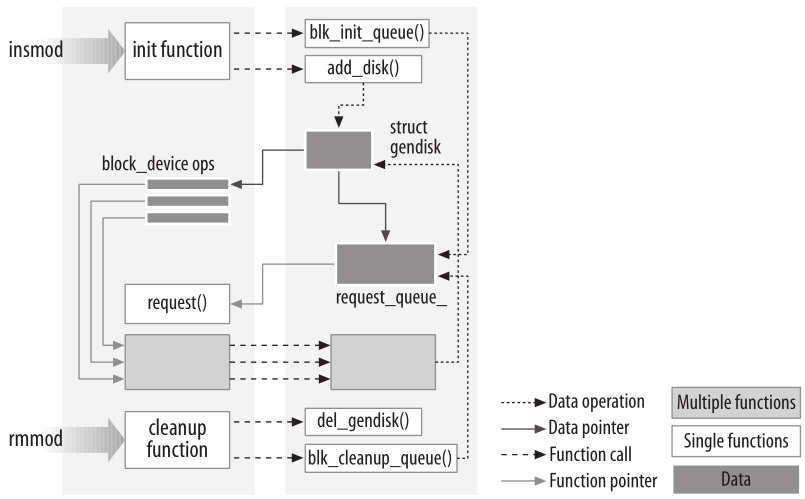
\includegraphics[width=\textwidth]{LinkingModule} \tiny{\cite{LinuxDrivers}}}
		\end{column}
		\begin{column}{.15\textwidth}
		\end{column}
	\end{columns}
\end{frame}


\begin{frame}[fragile]
	\frametitle{Verificar o Log do Linux}
	
	\begin{itemize}
		\item<1-> Verificar as informações do \textit{Log}:
	\end{itemize}

	\lstset{language=bash}
	\begin{block}<1->{}
	\begin{lstlisting}
		tail /var/log/syslog
		# OU
		tail /var/log/messages
	\end{lstlisting}
	\end{block}

	\pause
	
	\begin{itemize}
		\item<1-> Exemplo de conteúdo do \textit{Log}:
	\end{itemize}

	\lstset{language=TeX, numbers=none}
	\begin{lstlisting}
		Nov 11 15:38:35 debian-modulo kernel: Inicio do modulo.
		Nov 11 15:38:40 debian-modulo kernel: Fim do modulo.
	\end{lstlisting}

\end{frame}
